\section{Acceleration}\label{sectionAcceleration}
The acceleration is another important parameter in this project. It became important because in the start of the project, the agent has to learn how to accelerate itself. The agent with discrete actions didn't learn the right policy with having the acceleration as an trainable parameter. Acceleration was then changed from an trainable parameter to a constant parameter.

This was done to see if it was possible for the agent to learn how to drive a lap on different speed. This was done because it could be more realistic if it is possible to see the car driving faster than 10 km/h. The tested speed was with an interval of 20 km/h:
\begin{itemize}
	\item 10 km/h
	\item 30 km/h
	\item 50 km/h
\end{itemize} 

The way the car was driving these average speed, was first the car accelerate to a speed of 30 km/h example. After this then accelerating so the speed always stays at 30 km/h. The car will try to stay at this speed 30 km/h the whole lap. To accelerate it is the throttle in the environment which need to be changed.

To test the acceleration influence on the agent learning, all other parameters is as described in the introduction to this \Cref{cha:Result}. Thereby it should be possible to only see the influence on the acceleration.

The most important graph is the graph of the reward, which looks different from all the acceleration, this graph can be seen on \Cref{fig:change_of_acceleration_reward_graph}.


\begin{figure}[H]
	\centering
	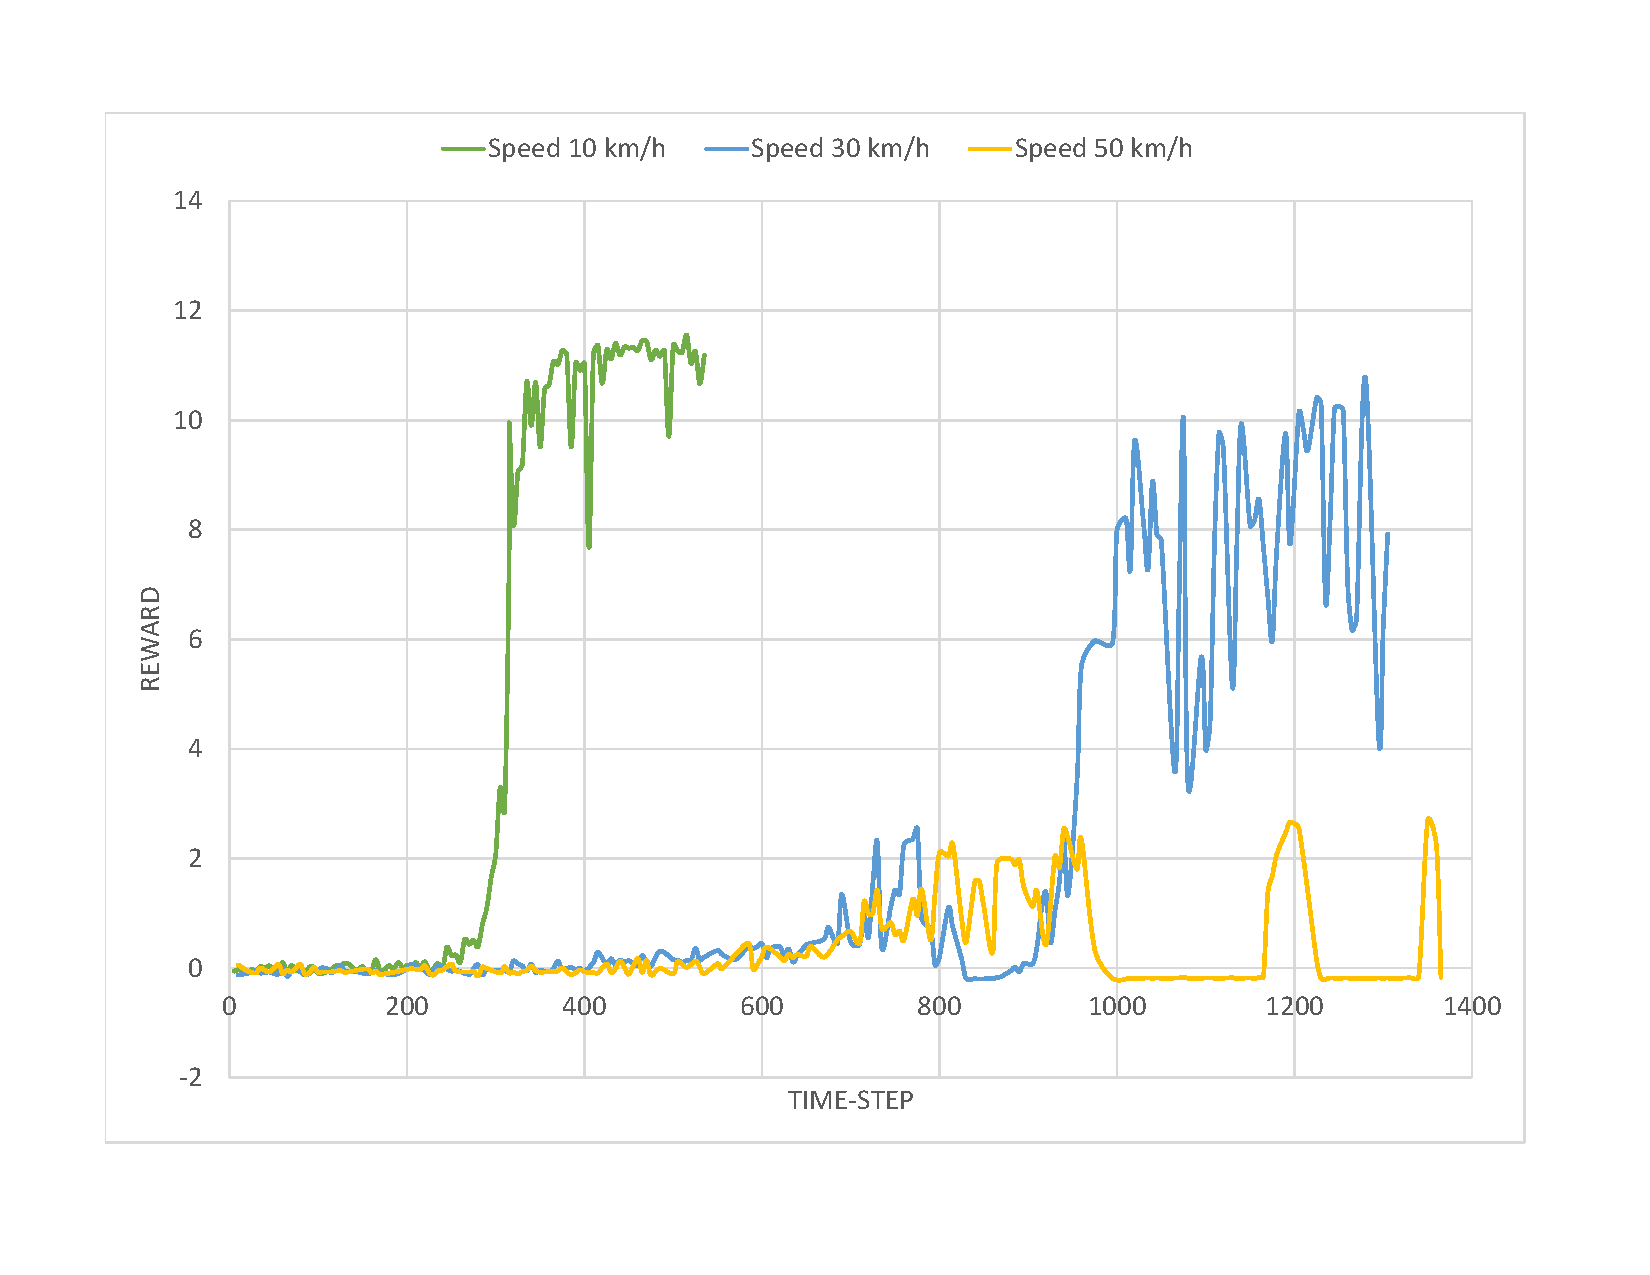
\includegraphics[width=1\textwidth]{Figures/Result/change_of_acceleration_reward_graph.pdf}
	\caption{Comparison of the three different speed with the reward getting from the environment}
	\label{fig:change_of_acceleration_reward_graph}
\end{figure} 


On \Cref{fig:change_of_acceleration_reward_graph} it is possible to see what happens with the different accelerations.   
 
\begin{figure}[H]
	\centering
	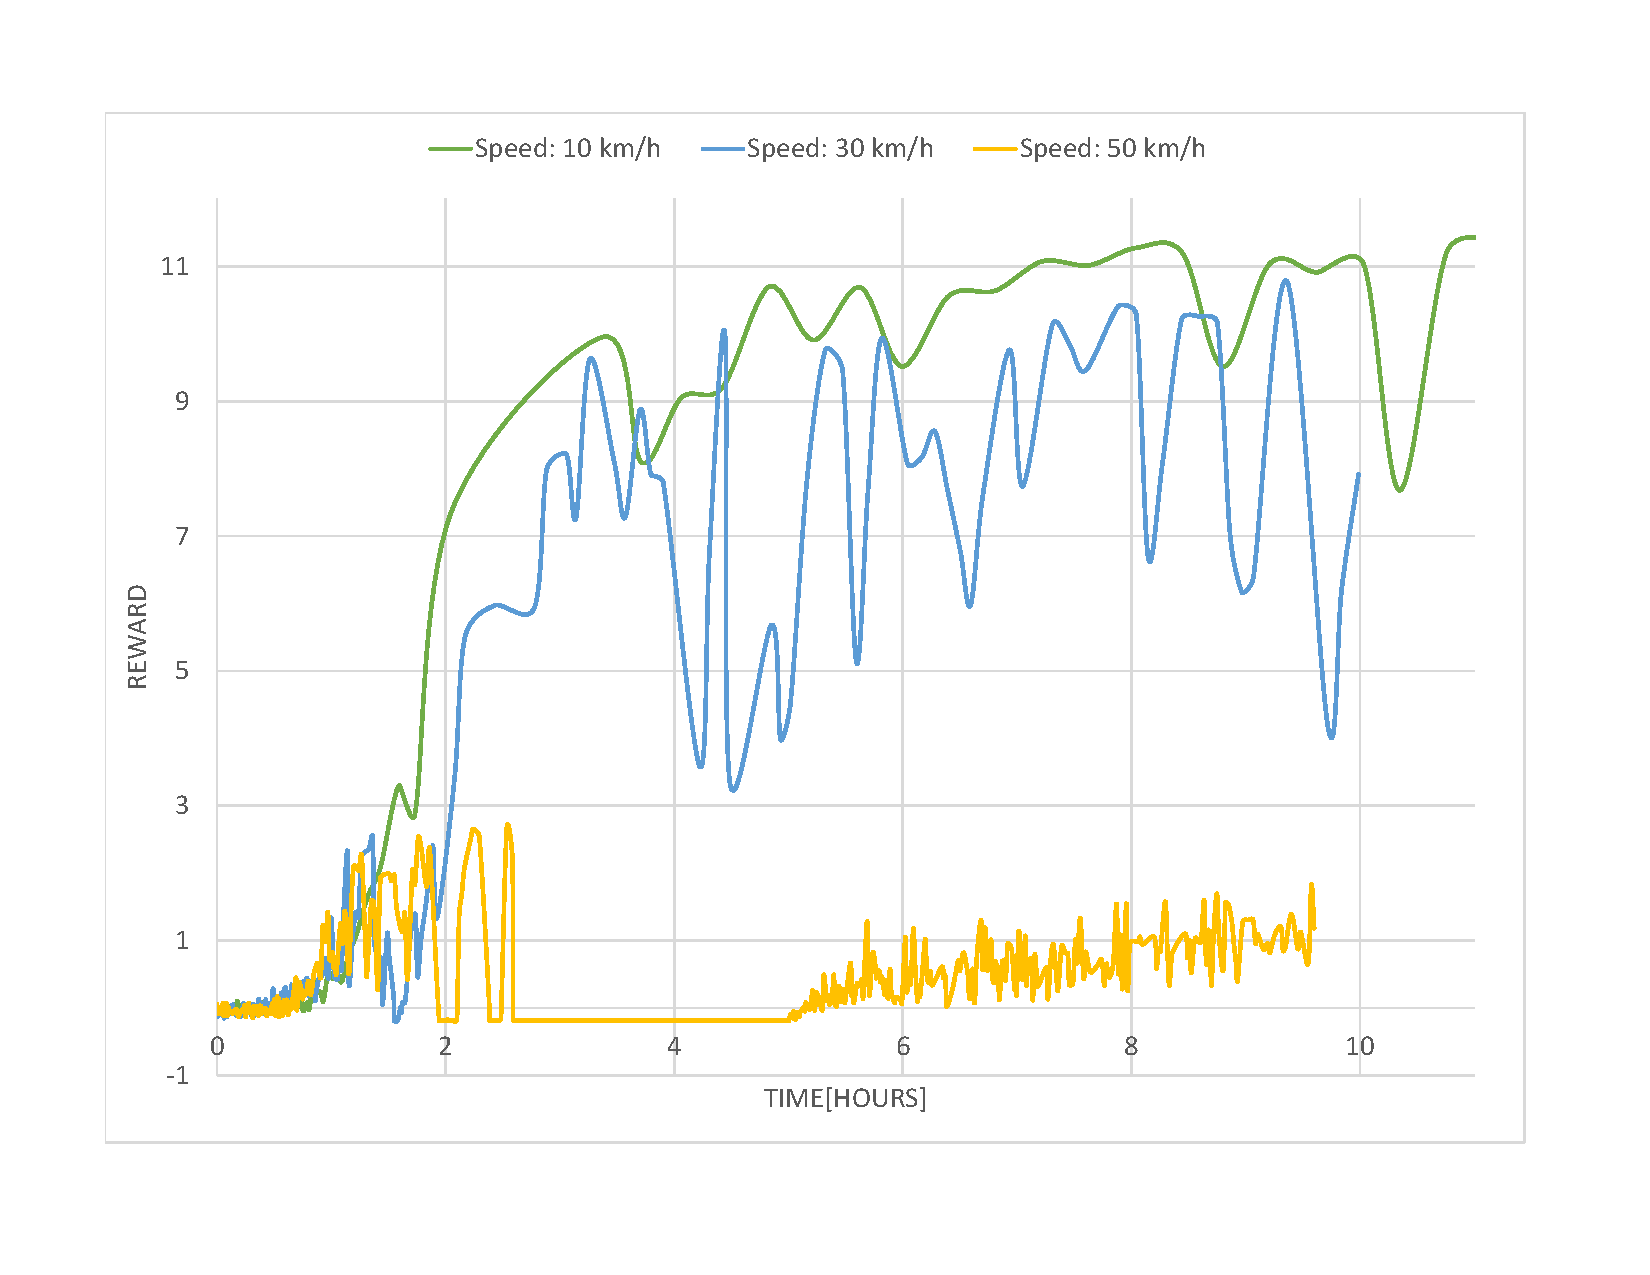
\includegraphics[width=1\textwidth]{Figures/Result/change_of_acceleration_reward_hours_graph.pdf}
	\caption{Comparison of the three different speed with the reward getting from the environment. Here it is the time in hours, instead of time-steps on the x-axis}
	\label{fig:change_of_acceleration_reward_hours_graph}
\end{figure}
  